\documentclass[11pt,class=report,crop=false]{standalone}
\usepackage[screen]{../python}



\begin{document}


%====================================================================
\chapitre{Statistics -- Data visualization}
%====================================================================

\objectifs{It's good to know how to calculate the minimum, maximum, average and quartiles of a series. It's even better to visualize them all on the same graph!}


%%%%%%%%%%%%%%%%%%%%%%%%%%%%%%%%%%%%%%%%%%%%%%%%%%%%%%%%%%%%%%%%
% Activity 1
%%%%%%%%%%%%%%%%%%%%%%%%%%%%%%%%%%%%%%%%%%%%%%%%%%%%%%%%%%%%%%%%

\begin{activite}[Basic statistics]

\objectifs{Goal: calculate the main characteristics 
of a series of data: minimum, maximum, mean and standard deviation.}

In this activity \ci{mylist} refers to a list of numbers (integer or floating point numbers). 

\begin{enumerate}
  \item Write your own function \ci{mysum(mylist)} which calculates the sum of the elements of a given list.
  Compare your result with the function \ci{sum()} described below which already exists in \Python{}. Especially for an empty list, check that your result is $0$. 
  
  \index{sum@\ci{sum}}
  
  \begin{fonctionpython}[\ci{python : sum()}]
   Use: \ci{sum(mylist)}\\
   Input: a list of numbers\\
   Output: a number
  
  \medskip
     
  Example: \ci{sum([4,8,3])} returns \ci{15}
  \end{fonctionpython}   
  
  \emph{You can now use the function \ci{sum()} in your programs!}
  
  
  \item Write a function \ci{mean(mylist)} that calculates the average of the items in a given list (and returns $0$ if the list is empty). \index{average}
  
  \item Write your own function \ci{minimum(mylist)} that returns the smallest value of the items in a given list. Compare your result with the \Python{} function \ci{min()} described below (who can also calculate the minimum of two numbers).
  
  \index{min@\ci{min}}  
  
  \begin{fonctionpython}[\ci{python : min()}]
   Use: \ci{min(mylist)} \ or \ \ci{min(a,b)}\\
   Input: a list of numbers or two numbers\\
   Output: a number
  
  \medskip
     
   Example : 
  \begin{itemize}  
    \item \ci{min(12,7)} returns \ci{7}  
    \item \ci{min([10,5,9,12])} returns \ci{5}
  \end{itemize}    

  \end{fonctionpython}   
  
  \emph{You can now use the function \ci{min()}, and of course also the function \ci{max()} in your programs!}\index{max@\ci{max}} 
  
  \item The \defi{variance}\index{variance} of a data series $(x_1,x_2,\ldots,x_n)$ is defined as the average of the squares of deviations from the mean. That is to say:
  $$v = \frac{1}{n}\big((x_1-m)^2 + (x_2-m)^2 + \cdots + (x_n-m)^2\big)$$
  where $m$ is the average of $(x_1,x_2,\ldots,x_n)$.
  
  Write a function \ci{variance(mylist)} that calculates the variance of the elements in a list.
  
  For example, for the series $(6,8,2,10)$, the average is $m = 6.5$, the variance is
  $$v = \frac{1}{4} \big((6-6.5)^2 + (8-6.5)^2 + (2-6.5)^2 + (10-6.5)^2\big) = 8.75.$$
  
  \item The \defi{standard deviation}\index{standard deviation@standard deviation} of a series $(x_1,x_2,\ldots,x_n)$ is the square root of the variance:
  $$e = \sqrt{v}$$
  where $v$ is the variance. Program a function \ci{standard_deviation(mylist)}.
  With the example above we find $e = \sqrt{v} = \sqrt{8.75} = 2.95\ldots$
  
%The square root function \ci{sqrt()} is not available by default in \Python. To use it, you must call the module of mathematical functions by the command: \\
% \centerline{\ci{from math import *}}

  \item Here are the average monthly temperatures (in Celsius degrees) in London and Chicago.

{\small	  
  \mycenterline{\ci{temp_london = [4.9,5,7.2,9.7,13.1,16.6,18.7,18.2,15.5,11.6,7.7,5.6]}}  
  \mycenterline{\ci{temp_chicago = [-5,-2.7,2.8,9.2,15.2,20.7,23.5,22.6,18.4,12.1,4.8,-1.9]}}
}



  Calculate the average temperature over the year in London and then in Chicago. Calculate the standard deviation of the temperatures in London and then in Chicago. What conclusions do you draw from this? 

\end{enumerate}

\end{activite}



%%%%%%%%%%%%%%%%%%%%%%%%%%%%%%%%%%%%%%%%%%%%%%%%%%%%%%%%%%%%%%%%
%%%%%%%%%%%%%%%%%%%%%%%%%%%%%%%%%%%%%%%%%%%%%%%%%%%%%%%%%%%%%%%%

\begin{cours}[Graphics with tkinter]

\index{tkinter@\ci{tkinter}}
\index{module!tkinter@\ci{tkinter}}
\index{graphic}
\index{window@window}

To display this:
\begin{center}
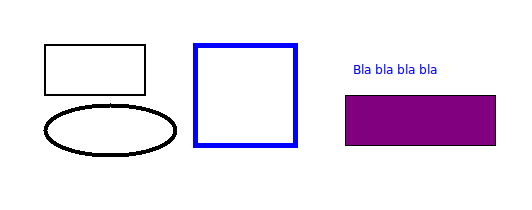
\includegraphics[scale=\myscale,scale=0.6]{screen-stat-lesson-intro}
\end{center}
The code is:
\begin{lstlisting}
# tkinter window
root = Tk()
        
canvas = Canvas(root, width=800, height=600, background="white")
canvas.pack(fill="both", expand=True)

# A rectangle
canvas.create_rectangle(50,50,150,100,width=2)

# A rectangle with thick blue edges
canvas.create_rectangle(200,50,300,150,width=5,outline="blue")

# A rectangle filled with purple
canvas.create_rectangle(350,100,500,150,fill="purple")

# An ellipse
canvas.create_oval(50,110,180,160,width=4)

# Some text
canvas.create_text(400,75,text="Bla bla bla bla",fill="blue")

# Launch of the window
root.mainloop()
\end{lstlisting}


Some explanations:
\begin{itemize}
  \item The \ci{tkinter} module allows us to define variables \ci{root} and \ci{canvas} that determine a graphic window (here width $800$ and height $600$ pixels).
  Then describe everything you want to add to the window. And finally the window is displayed by the command \ci{root.mainloop()} (at the very end). 
  
    
  \item Attention! The window's graphic marker has its $y$-axis pointing downwards. The origin $(0,0)$ is the top left corner (see figure below). 
  
  \item Command to draw a rectangle: \ci{create_rectangle(x1,y1,x2,y2)}; just specify the coordinates $(x_1,y_1)$, $(x_2,y_2)$ of two opposite vertices. The option \ci{width} adjusts the thickness of the line, \ci{outline} defines the color of this line, \ci{fill} defines the filling color.
  
  \item An ellipse is traced by the command \ci{create_oval(x1,y1,x2,y2)}, where $(x_1,y_1)$, $(x_2,y_2)$ are the coordinates of two opposite vertices of a rectangle framing the desired ellipse (see figure). A circle is obtained when the corresponding rectangle is a square!  
  
  \item Text is displayed by the command \ci{canvas.create_text(x,y,text="My text")} specifying the coordinates $(x,y)$ of the point from which you want to display the text. 
  
\end{itemize}

\myfigure{0.8}{
\tikzinput{fig-stat-lesson-intro}
}

\end{cours}


%%%%%%%%%%%%%%%%%%%%%%%%%%%%%%%%%%%%%%%%%%%%%%%%%%%%%%%%%%%%%%%%
% Activity 2
%%%%%%%%%%%%%%%%%%%%%%%%%%%%%%%%%%%%%%%%%%%%%%%%%%%%%%%%%%%%%%%%

\begin{activite}[Graphics]

\objectifs{Goal: visualize data by different types of graphs.}

\begin{center}
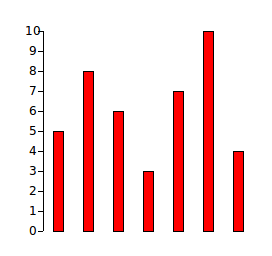
\includegraphics[scale=\myscale,width=5cm]{screen-stat-2a}\qquad\qquad
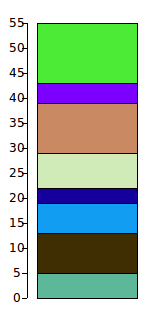
\includegraphics[scale=\myscale,height=5cm]{screen-stat-2b}

\qquad\qquad\textbf{Bar graphics}\qquad\qquad\qquad\quad
\textbf{Cumulative graph}
\end{center}

\begin{center}
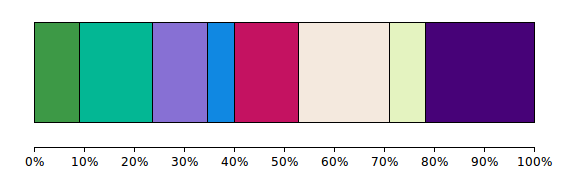
\includegraphics[scale=\myscale,width=7cm]{screen-stat-2c}\qquad\qquad
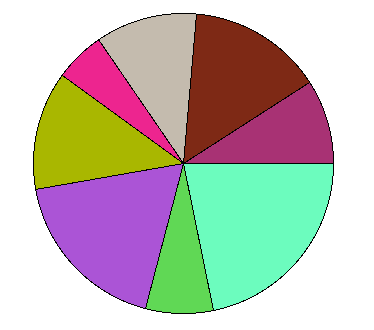
\includegraphics[scale=\myscale,width=4cm]{screen-stat-2d}

\qquad\textbf{Percentage graphics}\qquad\qquad\qquad\qquad\qquad\qquad
\textbf{Sector graph}
\end{center}

\begin{enumerate}
  \item \textbf{Bar graphics.} Write a function \ci{bar_graphics(mylist)} that displays the values of a list as vertical bars.
  


 \emph{Hints.}
  \begin{itemize}
    \item First of all, don't worry about drawing the vertical axis of the coordinates with the figures.
    \item You can define a variable \ci{scale} that allows you to enlarge your rectangles, so that they have a size adapted to the screen.
    \item If you want to test your graph with a random list, here is how to build a random list of $10$ integers between $1$ and $20$ :
    
\begin{lstlisting}
from random import *
mylist = [randint(1,20) for i in range(10)]
\end{lstlisting}

\end{itemize}

  \item \textbf{Cumulative graph.} Write a function \ci{cumulative_graphics(mylist)} that displays the values of a list in the form of rectangles one above the other.
  

  
  \item \textbf{Graphics with percentage.} Write a function \ci{percentage_graphics(mylist)} that displays the values of a list in a horizontal rectangle of fixed size (for example $500$ pixels) and is divided into sub-rectangles representing the values.
  


  \item \textbf{Sector graphics.} Write a function \ci{sector_graphics(mylist)} that displays the values of a list as a fixed size disk divided into sectors representing the values. 
 
The \ci{create_arc()} function, which allows you to draw arcs of circles, is not very intuitive. It is necessary to think that we draw a circle, by specifying the coordinates of the corners of a square which surrounds it, then by specifying the starting angle and the angle of the sector (in degrees). 

\mycenterline{\ci{canvas.create_arc(x1,y1,x2,y2,start=start_angle,extent=my_angle)}}


\myfigure{1}{
\tikzinput{fig-stat-arc}
}
The option \ci{style=PIESLICE} displays a sector instead of an arc. 


  \item \textbf{Bonus.} Gather your work into a program that allows the user to choose the diagram he wants by clicking on buttons, and also the possibility to get a new random series of data. \emph{To create and manage buttons with \ci{tkinter}, see the lesson below.}
  
\begin{center}
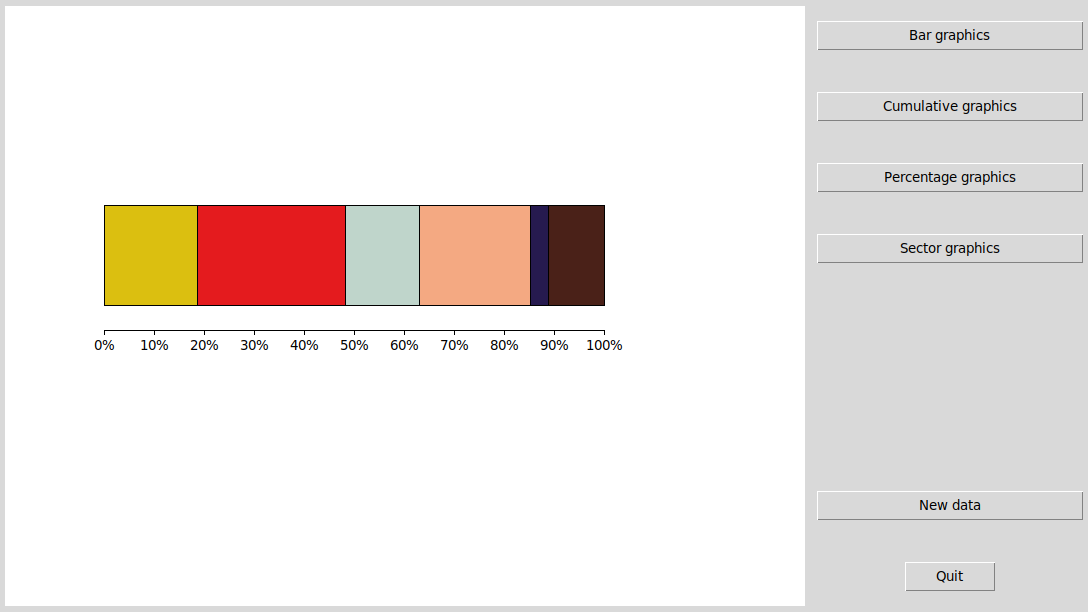
\includegraphics[scale=\myscale,scale=0.3]{screen-stat-2e-en}
\end{center} 
  
  \end{enumerate}
\end{activite}


%%%%%%%%%%%%%%%%%%%%%%%%%%%%%%%%%%%%%%%%%%%%%%%%%%%%%%%%%%%%%%%%
%%%%%%%%%%%%%%%%%%%%%%%%%%%%%%%%%%%%%%%%%%%%%%%%%%%%%%%%%%%%%%%%

\begin{cours}[Buttons with tkinter]

\index{button}

It is more ergonomic to display windows where actions are performed by clicking on buttons.
Here is the window of a small program with two buttons. The first button changes the color of the rectangle, the second button ends the program.
\begin{center}
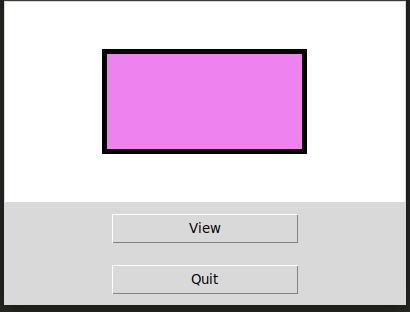
\includegraphics[scale=\myscale,scale=0.6]{screen-stat-lesson-buttons-en}
\end{center}

The code is:
\begin{lstlisting}
from tkinter import *
from random import *

root = Tk()     
canvas = Canvas(root, width=400, height=200, background="white")
canvas.pack(fill="both", expand=True)

def action_button():
    canvas.delete("all")      # Clear all
    colors = ["red","orange","yellow","green","cyan","blue","violet","purple"]
    col = choice(colors)      # Random color
    canvas.create_rectangle(100,50,300,150,width=5,fill=col)
    return

button_color = Button(root,text="View", width=20, command=action_button)
button_color.pack(pady=10)

button_quit = Button(root,text="Quit", width=20, command=root.quit)
button_quit.pack(side=BOTTOM, pady=10)

root.mainloop()
\end{lstlisting}

Some explanations:
\begin{itemize}
  \item A button is created by the command \ci{Button}. The \ci{text} option customizes the text displayed on the button. The button created is added to the window by the method \ci{pack}.
  \item The most important thing is the action associated with the button! It is the option \ci{command} that receives the name of the function to be executed when the button is clicked. For our example \ci{command=action_button}, associate the click on the button with a change of color.
  
  \item Attention! You have to give the name of the function without brackets: \ci{commande=my_function} and not \ci{command=my_function()}.
  
  \item To associate the button with \og{}Quit\fg{} and close the window, the argument is \ci{command=root.quit}.
  
  \item The instruction \ci{canvas.delete("all")} deletes all drawings from our graphic window.
  
\end{itemize}
\end{cours}


%%%%%%%%%%%%%%%%%%%%%%%%%%%%%%%%%%%%%%%%%%%%%%%%%%%%%%%%%%%%%%%%
% Activity 3
%%%%%%%%%%%%%%%%%%%%%%%%%%%%%%%%%%%%%%%%%%%%%%%%%%%%%%%%%%%%%%%%

\begin{activite}[Median and quartiles]

\objectifs{Goal: calculate the median and quartiles of some data.}

\begin{enumerate}
  \item Program a function \ci{median(mylist)}\index{median} which calculates the median value of the items of a given list. By definition, half of the values are less than or equal to the median, the other half are greater than or equal to the median.

  \emph{Background.} We note $n$ the length of the list and we assume that the list is ordered (from the smallest to the largest element).
  \begin{itemize}
    \item \textbf{Case $n$ odd.} The median is the value of the list at the rank $\frac{n-1}{2}$.    
    Example with \ci{mylist = [12,12,14,15,19]}:
    \begin{itemize}
      \item the length of the list is $n=5$ (indices range from $0$ to $4$),
      \item the middle index is the rank $2$,
      \item the median is the value \ci{mylist[2]}, so it is $14$.
    \end{itemize}
    
    \item \textbf{Case $n$ even.} The median is the average between the value of the list at rank $\frac{n}{2}-1$ and rank $\frac{n}{2}$.
    Example with \ci{mylist = [10,14,19,20]}:
    \begin{itemize}
      \item the length of the list is $n=4$ (indices range from $0$ to $3$),
      \item the middle indices are $1$ and $2$,
      \item the median is the average between \ci{mylist[1]} and \ci{mylist[2]}, so it is $\frac{14+19}{2} = 16.5$.
    \end{itemize}    
   \end{itemize} 
   
   
   
     
    \item The results of a class are collected in the following form of a number of students per grade:   
    \mycenterline{\ci{grade_count = [0,0,1,2,5,2,3,5,4,1,2]}} 
    
    The rank $i$ range is from $0$ to $10$. And the value at rank $i$ indicates the number of students who received the grade $i$.
    For example here, $1$ student got the grade $2$, $2$ students got the grade $3$, $5$ students got $4$, \ldots{}  
    Write a \ci{grades_to_list(grade_count)} function that takes the numbers of students for each grade as input and returns the list of all grades. For our example the function must return \ci{[2,3,3,4,4,4,4,4,5,5,6,6,6,7,...]}.

%[2, 3, 3, 4, 4, 4, 4, 4, 5, 5, 6, 6, 6, 7, 7, 7, 7, 7, 8, 8, 8, 8, 9, 10, 10]

       
    Deduce a function that calculates the median of a class's scores from the numbers of students for each grade.
    
    \item Write a function \ci{quartiles(mylist)} that calculates the quartiles $Q_1$, $Q_2$, $Q_3$ of the items in a given list. The quartiles\index{quartiles} divide the values into: one quarter below $Q_1$, one quarter between $Q_1$ and $Q_2$, one quarter between $Q_2$ and $Q_3$, one quarter above $Q_3$.
    For the calculation, we will use that:
    \begin{itemize}
      \item $Q_2$ is simply the median of the entire list (assumed ordered),
      \item $Q_1$ is the median of the sublist formed by the first half of the values,
      \item $Q_3$ is the median of the sublist formed by the second half of the values. 
    \end{itemize}           
\end{enumerate}

  For the implementation, it is necessary to discuss again whether the length $n$ of the list is even or not.
  
  Deduce a function that calculates the quartiles of a class's grades from a list of a number of students per grade.

\end{activite}


%%%%%%%%%%%%%%%%%%%%%%%%%%%%%%%%%%%%%%%%%%%%%%%%%%%%%%%%%%%%%%%%
% Activity 4
%%%%%%%%%%%%%%%%%%%%%%%%%%%%%%%%%%%%%%%%%%%%%%%%%%%%%%%%%%%%%%%%

\begin{activite}[Box plot]

\objectifs{Goal: drawing box plots.}

A \defi{box plot} is a diagram that represents the main characteristics of a statistical series: minimum, maximum, median and quartiles. The schematic diagram is as follows:

\myfigure{0.45}{
  \tikzinput{fig-stat-boite}
} 

Write a \ci{box_plot(grade_count)} function that draws the box plot of a class's grades from a list of a number of students per grade (see previous activity).

\begin{center}
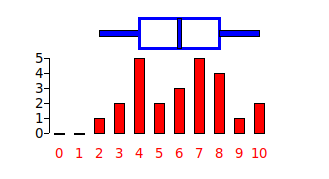
\includegraphics[scale=\myscale,scale=0.7]{screen-stat-4-en}
\end{center}

	
\end{activite}



%%%%%%%%%%%%%%%%%%%%%%%%%%%%%%%%%%%%%%%%%%%%%%%%%%%%%%%%%%%%%%%%
% Activity 5
%%%%%%%%%%%%%%%%%%%%%%%%%%%%%%%%%%%%%%%%%%%%%%%%%%%%%%%%%%%%%%%%

\begin{activite}[Moving average]

\objectifs{Goal: calculate moving averages in order to draw \og{}smooth\fg{} curves.}

\index{average}

\begin{enumerate}
  \item Simulates the stock market price of the index \emph{NISDUQ} over 365 days.
  At the beginning, the day $j=0$, the index is equal to $1000$. Then the index for a day is determined by adding a random value (positive or negative) to the value of the previous day's index:  
  \mycenterline{index of the day $j$ = index of the day $(j-1)$ \ + \ random value.}
  
  For this random value, you can try a formula like:  
  \mycenterline{\ci{value = randint(-10,12)/3}}
  
  Write a function \ci{index_stock_exchange()}, without parameter, which returns a list of $365$ index values using this method.
  
  \item Trace point by point the index curve over a year. (To draw a point, you can display a square with a size of $1$ pixel.)
  
\begin{center}
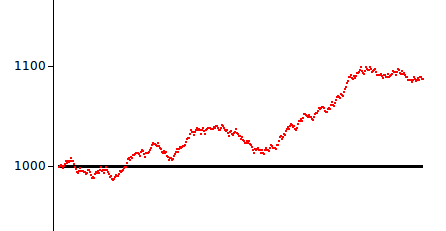
\includegraphics[scale=\myscale,scale=0.7]{screen-stat-5a}
\end{center}

   \item \emph{Since the daily index curve is very chaotic, we want to smooth it out in order to make it more readable. For this we calculate moving averages.}
   
   The moving average at $7$ days for the day $j$, is the average of the last $7$ indices. For example: the moving average (at $7$ days) for the day $j = 7$ is the average of the day's indices $j=1,2,3,4,5,6,7$. You can change the duration: for example the moving average at $30$ days is the average of the last $30$ indices.
   
   Write a function \ci{moving_average(mylist,duration)} that returns a list of all moving averages in a data set with respect to a fixed time.
   
    \item Trace point by point on the same graph: the index curve over a year\couleurnb{ (in red below)}{}, the moving average curve at $7$ days\couleurnb{  (in blue below)}{} and the moving average curve at $30$ days\couleurnb{ (in brown below)}{}. Note that the longer the duration, the more the curve is \og{}smooth\fg{}. (Of course the moving average curve at $30$ days only starts from the thirtieth day.)
   
\begin{center}
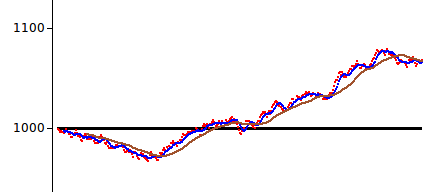
\includegraphics[scale=\myscale,scale=0.8]{screen-stat-5b}
\end{center}

\end{enumerate}

\end{activite}


\end{document}
